\documentclass[11pt,a4paper,oneside]{article}\usepackage[]{graphicx}\usepackage[]{color}
%% maxwidth is the original width if it is less than linewidth
%% otherwise use linewidth (to make sure the graphics do not exceed the margin)
\makeatletter
\def\maxwidth{ %
  \ifdim\Gin@nat@width>\linewidth
    \linewidth
  \else
    \Gin@nat@width
  \fi
}
\makeatother

\definecolor{fgcolor}{rgb}{0.345, 0.345, 0.345}
\newcommand{\hlnum}[1]{\textcolor[rgb]{0.686,0.059,0.569}{#1}}%
\newcommand{\hlstr}[1]{\textcolor[rgb]{0.192,0.494,0.8}{#1}}%
\newcommand{\hlcom}[1]{\textcolor[rgb]{0.678,0.584,0.686}{\textit{#1}}}%
\newcommand{\hlopt}[1]{\textcolor[rgb]{0,0,0}{#1}}%
\newcommand{\hlstd}[1]{\textcolor[rgb]{0.345,0.345,0.345}{#1}}%
\newcommand{\hlkwa}[1]{\textcolor[rgb]{0.161,0.373,0.58}{\textbf{#1}}}%
\newcommand{\hlkwb}[1]{\textcolor[rgb]{0.69,0.353,0.396}{#1}}%
\newcommand{\hlkwc}[1]{\textcolor[rgb]{0.333,0.667,0.333}{#1}}%
\newcommand{\hlkwd}[1]{\textcolor[rgb]{0.737,0.353,0.396}{\textbf{#1}}}%

\usepackage{framed}
\makeatletter
\newenvironment{kframe}{%
 \def\at@end@of@kframe{}%
 \ifinner\ifhmode%
  \def\at@end@of@kframe{\end{minipage}}%
  \begin{minipage}{\columnwidth}%
 \fi\fi%
 \def\FrameCommand##1{\hskip\@totalleftmargin \hskip-\fboxsep
 \colorbox{shadecolor}{##1}\hskip-\fboxsep
     % There is no \\@totalrightmargin, so:
     \hskip-\linewidth \hskip-\@totalleftmargin \hskip\columnwidth}%
 \MakeFramed {\advance\hsize-\width
   \@totalleftmargin\z@ \linewidth\hsize
   \@setminipage}}%
 {\par\unskip\endMakeFramed%
 \at@end@of@kframe}
\makeatother

\definecolor{shadecolor}{rgb}{.97, .97, .97}
\definecolor{messagecolor}{rgb}{0, 0, 0}
\definecolor{warningcolor}{rgb}{1, 0, 1}
\definecolor{errorcolor}{rgb}{1, 0, 0}
\newenvironment{knitrout}{}{} % an empty environment to be redefined in TeX

\usepackage{alltt}
\usepackage{amsmath,amsthm,amsfonts,amssymb}
\usepackage{pst-eucl,pstricks,pstricks-add}
%\usepackage[utf8]{inputenc}
%\usepackage[latin1]{inputenc}
\usepackage[spanish,activeacute]{babel}
\usepackage[a4paper,margin=2.5cm]{geometry}
\usepackage{times}
\usepackage[T1]{fontenc}
\usepackage{titlesec}
\usepackage{color}
\usepackage{url}
\usepackage{float}
\usepackage{cite}
\usepackage{graphicx}
\usepackage{multicol}
\usepackage{float}
\usepackage{lmodern}
\parindent=0mm
\IfFileExists{upquote.sty}{\usepackage{upquote}}{}
\begin{document}

\thispagestyle{empty}
{\sf
{\huge \scshape Escuela Polit\'{e}cnica Nacional} \\[5mm]
{\Large \scshape Facultad de Ciencias}\hfill \rule{0.05\textwidth}{0.5pt} {\scshape Deber 08} \rule{0.05\textwidth}{0.5pt}\\[8mm]
{\scshape Tema: Aplicaciones de la derivada}\\
}

\section{Puntos críticos}

\begin{enumerate}
      \item Encuentre los números críticos de las funciones dadas.
      \begin{multicols}{2}
      \begin{enumerate}
            \item $f(x)=2x^3-15x^2-36x$
            \item $f(x)=(x-2)^2(x-1)$
            %\item $f(x)=\displaystyle \frac{x^2}{x^2+2}$
            \item $f(x)=\displaystyle \frac{x+4}{\sqrt[3]{x+1}}$
            %\item $f(x)=\cos(4x)$
            \item $f(x)=e^{-x}+2x$
      \end{enumerate}
      \end{multicols}
      
      \item Encuentre los extremos absolutos de la función dada sobre el intervalo indicado.
      \begin{multicols}{2}
      \begin{enumerate}
            \item $f(x)=x^3-6x^2+2$;\quad $[-3,2]$
            \item $f(x)=x^4(x-1)^2$;\quad $[-1,2]$
            \item $f(x)=\displaystyle \frac{\sqrt{x}}{x^2+1}$;\quad $[\frac{1}{4}, \frac{1}{2}]$
            \item $f(x)=3+2\sen^2 (24x)$;\quad $[0, \pi]$
      \end{enumerate}
      \end{multicols}
\end{enumerate}

\section{Teorema de Rolle}

\begin{enumerate}
      \item Determine si la función dada satisface las hipótesis del teorema de Rolle sobre el intervalo indicado. En caso afirmativo, encuentre todos los valores de $c$ que satisfacen la conclusión del teorema.
      \begin{multicols}{2}
      \begin{enumerate}
            \item $f(x)=x^2-4$;\quad $[-2,2]$
            \item $f(x)=x^3-5x^2+4x$;\quad $[0,4]$
            \item $f(x)=x(x-1)^2$;\quad $[0,1]$
            \item $f(x)=\tan x$;\quad $[0,\pi]$
      \end{enumerate}
      \end{multicols}
\end{enumerate}

\section{Gráficas de funciones}

\begin{enumerate}
      \item Use la prueba de la primera derivada para encontrar los extremos relativos de la función dada.
      Grafique.
      \begin{multicols}{2}
      \begin{enumerate}
            \item $f(x)=x^3+x-3$
            \item $f(x)=(x^2-4)^{2/3}$
            \item $f(x)=x\sqrt{1-x^2}$
            \item $f(x)=\displaystyle \frac{x^2}{x^2-4}$
      \end{enumerate}
      \end{multicols}
      
      \item Use la segunda derivada para determinar los intervalos sobre los cuales la gráfica de la función es cóncava y los intervalos sobre los cuales es convexa. Grafique.
      \begin{multicols}{2}
      \begin{enumerate}
            \item $f(x)=x^{1/3}+2x$
            \item $f(x)=(x+5)^3$
            \item $f(x)=\sqrt{x^2+10}$
            \item $f(x)=\displaystyle \frac{x-1}{x+2}$
      \end{enumerate}
      \end{multicols}
\end{enumerate}

\section{Optimización}

\begin{enumerate}
      \item Encuentre dos números positivos cuyo producto sea 50 y cuya suma sea mínima.
      \item Encuentre el o los puntos sobre la gráfica $y^2=6x$ más próximo a $(5,0)$.
      \item Un granjero tiene 3000 metros de cerca a la mano. Determine las dimensiones de un corral rectangular que contenga el área máxima.
      \item Encuentre las dimensiones del cilindro circular recto con volumen máximo que puede inscribirse en un cono circular recto de 8 cm de radio y 12 cm de altura.
      \item Una persona desea cortar una pieza de 1 m de longitud de alambre en dos partes. Una parte debe doblarse en forma de círculo y la otra en forma de cuadrado. ?`Cómo debe cortarse el alambre de modo que la suma de las áreas sea máxima?
      \item Se producirá una caja, abierta por la parte superior, de una pieza cuadrada de cartón cortando un cuadrado de cada esquina y doblando los lados. Los cuadrados blancos se han cortado y el cartón se ha doblado a lo largo de las líneas discontinuas. Dado que la pieza de cartón mide 40 cm por lado, encuentre las dimensiones de la caja con que se obtiene el volumen máximo. ?`Cuál es el volumen máximo?
      
      \begin{figure}[H]
      \centering
      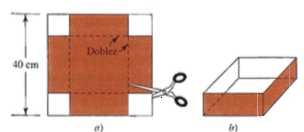
\includegraphics[scale=.7]{images/fig01.png}
      \end{figure}
      
      \item Dos astabanderas están aseguradas con cables sujetos a un solo punto entre las astas. ?`Dónde debe ubicarse el punto a fin de minimizar la cantidad de cable usado?
      
      \begin{figure}[H]
      \centering
      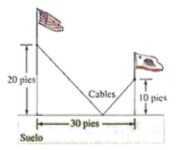
\includegraphics[scale=.7]{images/fig02.png}
      \end{figure}
      
      \item La pista de carreras que se muestra debe constar de dos partes rectas paralelas y dos partes semicirculares. La longitud de la pista debe medir 2 km. Encuentre el diseño de la pista de modo que el terreno rectangular encerrado por la pista sea máximo.
      
      \begin{figure}[H]
      \centering
      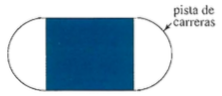
\includegraphics[scale=.7]{images/fig03.png}
      \end{figure}
      
      \item Se va a construir una tubería desde una refinería  a través de un pantano hasta tanques de almacenamiento. El costo de construcción es 25000 dólares por milla sobre el pantano y 20000 dólares por milla sobre tierra. ?`Cómo debe construirse la tubería para que el costo de producción sea mínimo?
      
      \begin{figure}[H]
      \centering
      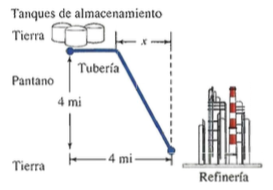
\includegraphics[scale=.7]{images/fig04.png}
      \end{figure}
      
      \item Una esquina de una hoja de papel de 8.5 pulgadas $\times$ 11 pulgadas se dobla sobre el otro  borde del papel como se muestra en la figura. Encuentre el ancho $x$ del doblez de modo que la longitud $L$ del pliegue sea mínima.
      
      \begin{figure}[H]
      \centering
      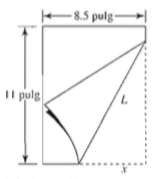
\includegraphics[scale=.7]{images/fig05.png}
      \end{figure}
      
\end{enumerate}

\end{document}
